% =====================================================================
\section{Analysis}
\label{sec:analysis}
% =====================================================================

% ---------------------------------------------------------------------
\subsection{Task 1: Business ecosystem}
\label{sec:t1}
% ---------------------------------------------------------------------

\citet[Def.~4.1]{OverbyAudestad2021} define the digital economy ecosystem as the relations and dependencies between digital services, ICT infrastructures, digital markets and authorities in a socioeconomic context. In line with Moore's original idea of business ecosystems, which the textbook builds on, Nord Pool's ecosystem crosses industries: it spans financial markets, electricity grids, ICT and government. Table~\ref{tab:stakeholders} identifies the direct and indirect stakeholders. Figure~\ref{fig:ecosystem} maps the most important dependencies using the textbook's notation for one-way and mutual dependence \citep[Fig.~4.3]{OverbyAudestad2021}.

\begin{table}[ht]
\centering
\small
\caption{Direct and indirect stakeholders in the Nord Pool ecosystem.}
\label{tab:stakeholders}
\begin{tabularx}{\textwidth}{L{3.3cm} L{1.4cm} Y Y}
\toprule
\textbf{Actor} & \textbf{Type} & \textbf{Role} & \textbf{Key dependency} \\
\midrule
Nord Pool AS & Platform & Day-ahead and intraday markets, central counterparty, market data & Needs TSO capacities, members' liquidity, Euronext's capital and technology \\
Euronext (66\%) & Direct & Capital, exchange technology, futures market and clearing house (from 2026) & Earns revenue from Nord Pool; its futures are based on the Nordic system price \\
Statnett, Svenska kraftnät, EPSO-G (34\% via TSO Holding) & Direct & Owners; supply cross-zonal capacities; operate grids & Depend on market coupling to allocate capacity \\
Fingrid, Energinet and other coupling TSOs & Direct & Supply capacities; no ownership since 2022 & Essential input without an ownership voice \\
Market participants (about 400 firms) & Direct & Generators, retailers, industrials, traders, aggregators & Need liquidity and guaranteed settlement \\
EPEX SPOT and other NEMOs & Direct & Competitors for members since 2020; partners in SDAC & Coopetition in the shared coupling \\
Regulators (national, ACER, EU) & Direct & NEMO designation, CACM rules, REMIT surveillance, cybersecurity rules & Set the rules of the game \\
Households and firms on spot contracts & Indirect & Pay prices formed on the platform & No influence over the platform \\
Futures traders (Euronext, EEX) & Indirect & Hedge using system-price contracts & Depend on the credibility of the system price \\
Data users & Indirect & Retailers, analysts, researchers, app developers & Depend on access to price data \\
Owner states and Euronext shareholders & Indirect & Owners of the partners & Indirect financial and policy interest \\
\bottomrule
\end{tabularx}
\end{table}

\textbf{Direct stakeholders.} The platform itself is Nord Pool AS, which runs the day-ahead and intraday markets, acts as central counterparty for all trades and sells market data \citep{NPAbout,NPClearing}. The two alliance partners contribute different resources. Euronext provides capital, exchange technology and financial distribution, and since March 2026 also operates a Nordic power futures market and the associated clearing house \citep{Euronext2026}. The TSOs provide something no other actor can supply: the cross-zonal transmission capacities that the price calculation requires. Market participants supply the bids and therefore the liquidity. EPEX SPOT, which entered the Nordic day-ahead market in 2020, is both a competitor for members and a partner in the shared European day-ahead coupling \citep{EPEX2020}. Regulators designate exchanges as nominated electricity market operators (NEMOs), set the coupling rules under the CACM guideline \citep{CACM2015} and supervise market integrity.

\textbf{Indirect stakeholders.} Households and firms on spot-price contracts are affected by every auction without taking part in it. Futures traders depend on the Nordic system price, which Nord Pool calculates and which most standard financial contracts in the Nordic region use as their reference price \citep{NPPrice}. Data users, from electricity retailers to researchers, buy or reuse Nord Pool's price data \citep{NPData,ERR2022}. The states that own the TSOs, and Euronext's shareholders, are indirect stakeholders through ownership.

% Figure 1: Ecosystem map (dependency notation after Øverby & Audestad, Fig. 4.3)
\begin{figure}[ht]
\centering
\begin{tikzpicture}[
  font=\footnotesize,
  box/.style={draw, rounded corners=2pt, align=center, text width=3.3cm, minimum height=1.0cm, fill=white},
  core/.style={box, text width=2.8cm, fill=blue!8, draw=blue!60!black, line width=0.8pt},
  partner/.style={box, fill=orange!10, draw=orange!70!black},
  ind/.style={box, text width=2.5cm, fill=gray!8, draw=gray!60, dashed},
  dep/.style={-{Stealth[length=2.2mm]}, thick},
  mut/.style={{Stealth[length=2.2mm]}-{Stealth[length=2.2mm]}, thick},
  lbl/.style={font=\scriptsize, fill=white, inner sep=1pt, align=center}
]
% core column
\node[core] (np)   at (0,0.9)   {\textbf{Nord Pool AS}\\day-ahead, intraday,\\CCP, data};
\node[box]  (epex) at (0,-1.4)  {\textbf{EPEX SPOT}\\(other NEMOs)};
\node[font=\scriptsize\itshape, text=blue!50!black] (sdaclbl) at (0,-2.3) {SDAC: shared coupling};
\begin{scope}[on background layer]
  \node[draw=blue!50, dashed, rounded corners=4pt, fill=blue!3, inner sep=6pt,
        fit=(np)(epex)(sdaclbl)] (sdac) {};
\end{scope}
\node[box, text width=4.4cm] (reg) at (0,3.5) {\textbf{Regulators}\\NEMO designation, CACM,\\REMIT, NIS2/NCCS};

% left column
\node[partner] (eur) at (-5.5,0.9)  {\textbf{Euronext} (66\%)\\capital, technology,\\futures, clearing};
\node[box]     (mem) at (-5.5,-1.4) {\textbf{Market participants}\\(about 400 firms)};

% right column: all TSOs
\node[partner] (tso)  at (5.5,0.9)  {\textbf{Owner TSOs} (34\%)\\Statnett,\\Svenska kraftnät,\\Litgrid (via EPSO-G)};
\node[box]     (ntso) at (5.5,-1.4) {\textbf{Non-owner TSOs}\\Fingrid, Energinet, \dots};
\begin{scope}[on background layer]
  \node[draw=orange!60!black, dotted, rounded corners=4pt, inner sep=5pt, fit=(tso)(ntso)] (tsos) {};
\end{scope}

% bottom row: indirect stakeholders
\node[ind] (cons) at (-5.5,-4.6) {Households and firms on spot contracts};
\node[ind] (fut)  at (-2.4,-4.6) {Futures traders\\(Euronext, EEX)};
\node[ind] (data) at (2.4,-4.6)  {Data users};
\node[ind] (own)  at (5.5,-4.6)  {Owner states;\\Euronext shareholders};

% dependencies: A -> B means "A depends on B"
\draw[mut] (eur) -- node[lbl, above=2pt]{ownership $\leftrightarrow$\\technology, capital} (np);
\draw[dep] (np.east) -- node[lbl, above=2pt]{capacity data for\\area prices (all TSOs)} (tsos.west |- np.east);
\draw[dep] (ntso) -- node[lbl, above=2pt]{depend on\\coupling} (ntso -| sdac.east);
\draw[mut] (mem) -- node[lbl, above=2pt]{liquidity $\leftrightarrow$\\settlement} (mem -| sdac.west);
\draw[dep] (np) -- node[lbl, right]{designation} (reg);
\draw[dep] (cons) -- node[lbl, right]{price pass-through} (mem);
\draw[dep] (fut.north) -- node[lbl, pos=0.22]{system price} (np.south west);
\draw[dep] (data.north) -- node[lbl, pos=0.22]{price data} (np.south east);
\draw[dep, dotted] (own) -- node[lbl, right]{ownership interest} (tsos.south -| own);
\end{tikzpicture}
\caption{Ecosystem map of the Nord Pool alliance. An arrow from A to B means that A depends on B, and a double arrow means mutual dependence \citep[notation after][Fig.~4.3]{OverbyAudestad2021}. Orange boxes are alliance partners, and dashed boxes are indirect stakeholders. Nord Pool depends on all TSOs for the capacity data behind the area prices, while the TSOs depend on the shared SDAC coupling rather than on Nord Pool specifically.}
\label{fig:ecosystem}
\end{figure}


\textbf{Critical relationships and dependencies.} The most critical relationship is between Nord Pool and the TSOs, and it is asymmetric. Nord Pool cannot calculate a single price without the TSOs' capacity data. The TSOs, however, depend on the market coupling as a whole rather than on Nord Pool specifically: since the multi-NEMO arrangement went live in 2020, the same capacities are allocated through one common coupling in which EPEX also takes part \citep{EPEX2020}. The TSOs also collect the congestion income that arises when prices differ between zones \citep{EU2019943}. In the notation of Figure~\ref{fig:ecosystem}, Nord Pool depends on the TSOs, while the TSOs depend on the coupling.

\textbf{Complementarities.} The partners' contributions are complementary in the sense of \citet{Jacobides2018}: Euronext's commercial and technological capabilities are worth more when combined with the TSOs' system knowledge, legitimacy and data, and vice versa. A second complementarity links the spot and futures markets. Liquidity in the spot market makes the system price a credible reference, which supports the futures market that Euronext launched in March 2026 \citep{Euronext2026}. Even a competitor depends on this output: EEX uses ``the Nordic Elspot System Price as determined by NordPool'' as the underlying for its Nordic system price futures \citep{EEX2024}. Finally, Nord Pool and EPEX illustrate coopetition. They compete for the same members while cooperating on a common price calculation \citep[Def.~8.4]{OverbyAudestad2021}.

\textbf{How the alliance changes roles, incentives and influence.} The alliance has moved Nord Pool from a utility-like exchange owned by grid operators towards a commercial platform controlled by a listed group. Euronext's stated rationale for the acquisition was to diversify revenue, strengthen Oslo as its Nordic hub and ``reinforce our commodities franchise'' \citep{Euronext2020}. Several later decisions are consistent with this commercial logic. Historical price data was moved behind a paywall in 2022 \citep{ERR2022}. Retailers pay for licensed price data \citep{NPData}. Euronext acquired Nasdaq's Nordic power futures and relaunched them in the Nord Pool environment \citep{FOW2025,Euronext2026}.

The TSOs' influence has changed form rather than disappeared. Their 34\% stake translates into one of eight board seats. The chair is a Euronext executive, and four other shareholder-side members are listed with job titles but without stated employers \citep{NPBoard}. Fingrid and Energinet sold their stakes in TSO Holding in 2022 \citep{EPSOG2022}, yet their capacity data remain indispensable. TSO influence therefore runs mainly through regulation and the governance of the shared coupling, not through ownership. This creates a governance asymmetry: the actors that supply the critical input and carry the system risk have limited say over the platform's commercial choices. Regulators have consequently become more central ecosystem actors, as the textbook's description of authorities as watchdogs would predict \citep[Sect.~4.7]{OverbyAudestad2021}.

Finally, the ecosystem has been in what the textbook calls a transient rather than a stationary state \citep[Sect.~4.2]{OverbyAudestad2021}. Within six years it has gained a new controlling owner (2020), a competing exchange (2020), a new ownership mix in TSO Holding (2022), new capacity calculation (2024), new products (2025) and a new futures market (2026). Each change redistributed roles among the same core actors. Any assessment of the alliance is therefore a snapshot, and the balance of influence between Euronext and the TSOs is still evolving.

% ---------------------------------------------------------------------
\subsection{Task 2: Network effects and path dependency}
\label{sec:t2}
% ---------------------------------------------------------------------

A network effect is the effect that the number of users or the amount of usage of a service has on the value of that service as perceived by each user \citep[Def.~9.1]{OverbyAudestad2021}. The textbook stresses that this demand-side effect must be distinguished from supply-side economies of scale. The distinction matters for Nord Pool. An exchange has high fixed IT costs and close to zero marginal cost per trade, but that is a cost advantage of size, not a network effect. Table~\ref{tab:ne} summarises the network effects we identify.

\begin{table}[ht]
\centering
\small
\caption{Network effects associated with the Nord Pool platform.}
\label{tab:ne}
\begin{tabularx}{\textwidth}{L{3.2cm} L{3.4cm} L{2.0cm} Y}
\toprule
\textbf{Effect} & \textbf{Type} & \textbf{Sign, strength} & \textbf{Evidence / mechanism} \\
\midrule
Buyers $\leftrightarrow$ sellers & Cross-side, direct & +, strong & Liquidity: more counterparties give better prices and execution \citep{Pagano1989} \\
Sellers $\leftrightarrow$ sellers & Same-side, direct & $-$, weak & Price competition among sellers; offset by a more robust price \\
Market coupling (zones, TSOs) & Cross-side, indirect; shared by all NEMOs & +, strong & More zones widen the set of feasible trades \citep{Newbery2016} \\
Data accumulation & Data network effect, indirect & +, moderate & More trades produce a richer price history and more valuable data \citep{NPData} \\
Spot $\leftrightarrow$ futures & Cross-market, indirect & +, strong & A credible system price supports futures liquidity, and vice versa \citep{NPPrice,Euronext2026} \\
\bottomrule
\end{tabularx}
\end{table}

\textbf{Buyers and sellers.} The core effect is liquidity. Each additional seller improves the prices and execution available to buyers, and each additional buyer does the same for sellers. In the textbook's terms, this is a positive, direct, cross-side network effect \citep[Sect.~9.4--9.5]{OverbyAudestad2021}. \citet{Pagano1989} explains why such markets tend to concentrate: traders prefer the venue where others already trade, because liquidity lowers their trading costs. Same-side effects are mixed. More sellers increase competition, which is a weak negative effect for sellers, similar to sellers on eBay \citep[Sect.~10.3]{OverbyAudestad2021}. At the same time, more participants on both sides make the clearing price more robust.

\textbf{Institutions and data sources joining.} Value also grows as bidding zones, interconnectors and TSOs join, because every added zone widens the set of possible trades. \citet{Newbery2016} estimate substantial welfare gains from integrating European electricity markets. Crucially, this network belongs to the Single Day-Ahead Coupling (SDAC), not to Nord Pool: all NEMOs share one algorithm and one price per zone. EU regulation has in effect turned the strongest network effect in the market into a commons that competitors also enjoy. In addition, more trading produces a richer price history. Nord Pool sells data going back almost three decades \citep{NPData}, which is an indirect data network effect \citep[Sect.~9.3]{OverbyAudestad2021}.

\textbf{Complementary services.} A further effect links spot and futures. A liquid spot market makes the system price a credible reference, credible references attract hedging in futures, and hedging opportunities in turn attract spot participants. When Euronext migrated Nasdaq's Nordic futures in March 2026, 173~TWh of open interest and 86 participants moved to the new market \citep{Euronext2026}. EEX reported 20.41~TWh of open interest in its Nordic futures in July 2026 \citep{EEX2026}. The figures are from different dates, but they suggest that futures liquidity has concentrated at Euronext, which is tipping on the futures side.

\textbf{Negative network effects.} The same interconnection that creates value also transmits failures. The textbook notes that technical issues, interruptions and downtime can trigger negative network effects, in which users leaving a service prompt others to leave \citep[Sect.~9.2]{OverbyAudestad2021}. In a coupled market, a technical failure in one place can decouple several zones at once, as in the incidents of 2019 and 2021 \citep{NPIncident2019,SDAC2021}. Under multi-NEMO competition, repeated failures at one exchange could start such a spiral, because members can now move their trading to a competitor without leaving the coupled market. The network effects that protect Nord Pool's position therefore also make its operational reliability a competitive variable, a point we return to in Task~4.

\textbf{Path dependency and switching costs.} Path dependence means that a market's evolution depends on its initial state, network effects and external events, and can end in one of several equilibria \citep[Def.~11.2]{OverbyAudestad2021}. \citet{Arthur1989} shows how small early advantages can lock a market into one outcome. Nord Pool's start in 1996 gave it a first-mover position \citep{NPAbout}, and its system price became the reference for Nordic financial contracts \citep{NPPrice}. The system price is thus a de facto standard \citep[Def.~15.1]{OverbyAudestad2021}: every contract written against it makes a change of reference more costly. Members also face switching costs \citep[Def.~12.2]{OverbyAudestad2021} from IT integration, collateral arrangements, trained staff and access to historical data.

\textbf{Lock-in, tipping and winner-takes-all.} Before 2020, the Nordic spot market had effectively tipped to Nord Pool. Regulation has since deliberately lowered switching costs between exchanges. Under CACM, several NEMOs can operate in the same country, and the Nordic multi-NEMO arrangement went live on 3~June 2020 \citep{EPEX2020,CACM2015}. Common products, such as the 15-minute products introduced in SDAC from 1~October 2025 \citep{OTE2025}, make exchanges more interchangeable. This is the electricity-market equivalent of number portability, the textbook's example of regulation that reduces lock-in \citep[Sect.~12.6]{OverbyAudestad2021}. EPEX traded 54~TWh in the Nordic day-ahead market in 2024 \citep{EPEX2025}: a foothold rather than a takeover. We therefore characterise the spot market as a contestable incumbency rather than a winner-takes-all monopoly. Nord Pool's low day-ahead trading fee of €0.040/MWh \citep{NPFees2026} is consistent with competitive pressure, although we cannot establish causality.

Lock-in has not disappeared but may be moving. The system price, the historical data and the futures market are all controlled within the Euronext group, and they are less exposed to multi-NEMO competition than the auction itself. In terms of the lock-in cycle \citep[Sect.~12.4]{OverbyAudestad2021}, vertical integration from spot to futures can entrench participants who trade and hedge across both markets.

% ---------------------------------------------------------------------
\subsection{Task 3: Multisided platform mapping}
\label{sec:t3}
% ---------------------------------------------------------------------

\textbf{Is Nord Pool a multisided platform?} A multisided platform (MSP) enables direct interactions between two or more distinct user groups that are all affiliated with the platform \citep[Def.~10.1]{OverbyAudestad2021}, building on \citet{HagiuWright2015}. Nord Pool raises a classification problem. It acts as central counterparty for all trades \citep{NPClearing}, so formally it buys from every seller and sells to every buyer. This resembles the textbook's reseller, which is explicitly not an MSP \citep[Sect.~10.5]{OverbyAudestad2021}. However, buyers and sellers set their own prices and quantities, and Nord Pool takes no market position. For \citet{HagiuWright2015}, direct interaction means that the sides keep control over the key terms of their interaction. We therefore classify Nord Pool as an MSP in which central clearing is an added risk service, not a resale.

\textbf{The sides.} We identify five groups (Figure~\ref{fig:msp}):
\begin{enumerate}
  \item Sellers: hydro, wind, nuclear and thermal generators.
  \item Buyers: retailers and industrial consumers. Because many firms buy in some hours and sell in others, the first two sides are defined by function rather than identity.
  \item Small participants and aggregators, a distinct tier with its own tariff.
  \item Data customers: retailers, analysts, media and researchers who buy price data.
  \item Futures traders, an indirect side connected through the system price.
\end{enumerate}
TSOs are partners that supply a critical input rather than a paying side. Consumers are not a side at all, because they are not affiliated with the platform.

\textbf{Competition.} The textbook identifies three types of competition for MSPs \citep[Sect.~10.2.3]{OverbyAudestad2021}, and all three apply here. First, Nord Pool competes directly with another platform offering the same service, EPEX SPOT, for trading members. Second, it competes with different kinds of platforms for particular sides. On the data side, its competitor is the free ENTSO-E Transparency Platform. On the trading side, bilateral contracts outside the exchange compete for some of the volume. Third, users on the same side compete with each other, as generators do when they bid into the same auction. This layered competition limits how far Nord Pool can raise prices on any one side.

\textbf{Strength of the network effects.} The buyer--seller effect is strong and positive in both directions. Data customers benefit strongly from trading activity but have little effect on traders, so this effect runs one way. Small participants add depth and flexibility, which moderately benefits larger members. Among sellers, the same-side effect is weakly negative because of competition.

% Figure 2: Multisided platform map with network effects and prices
\begin{figure}[ht]
\centering
\begin{tikzpicture}[
  font=\footnotesize,
  side/.style={draw, rounded corners=2pt, align=center, text width=3.1cm, minimum height=1.25cm, fill=green!6, draw=green!40!black},
  plat/.style={draw, rounded corners=3pt, align=center, text width=3.6cm, minimum height=1.6cm, fill=blue!8, draw=blue!60!black, line width=0.8pt},
  partner/.style={draw, rounded corners=2pt, align=center, text width=3.8cm, minimum height=1.1cm, fill=orange!10, draw=orange!70!black, dashed},
  aff/.style={thick, gray!70},
  ne/.style={{Stealth[length=2mm]}-{Stealth[length=2mm]}, thick, red!65!black},
  ne1/.style={-{Stealth[length=2mm]}, thick, red!65!black},
  lbl/.style={font=\scriptsize, fill=white, inner sep=1pt, align=center}
]
\node[plat] (np) at (0,0) {\textbf{Nord Pool}\\matching, system price,\\central clearing};
\node[side] (sel) at (-4.8,0.9)  {\textbf{Sellers}\\(generators)\\\scriptsize €21.5k/yr + €0.055/MWh};
\node[side] (buy) at (4.8,0.9)   {\textbf{Buyers}\\(retailers, industrials)\\\scriptsize €21.5k/yr + €0.055/MWh};
\node[side] (sml) at (-4.8,-2.3) {\textbf{Small participants,}\\\textbf{aggregators}\\\scriptsize €0/yr + €0.140/MWh};
\node[side] (dat) at (4.8,-2.3)  {\textbf{Data customers}\\\scriptsize €600--3,500/yr};
\node[side] (fut) at (0,4.6)   {\textbf{Futures traders}\\(Euronext, EEX)\\\scriptsize pay Euronext/EEX, not Nord Pool};
\node[partner] (tso) at (0,-3.2) {\textbf{TSOs} (partner, input)\\capacity data; no trading fee};

% affiliation lines
\foreach \s in {sel,buy,sml,dat} \draw[aff] (\s) -- (np);
\draw[aff, dashed] (fut) -- node[lbl]{system price} (np);
\draw[aff, dashed, orange!70!black] (tso) -- node[lbl]{capacities} (np);

% network effects
\draw[ne] (sel.north) to[out=25,in=155] node[lbl, pos=0.5, yshift=1pt]{(+/+) strong cross-side} (buy.north);
\draw[ne] (sml.north) -- node[lbl, right]{(+/+) moderate:\\depth, flexibility} (sel.south);
\draw[ne1] (buy.south) -- node[lbl, right]{traders $\rightarrow$ data\\(+/0) one-way} (dat.north);
\draw[ne, red!50] (sel.west) to[out=150,in=210, looseness=5] node[lbl, left]{($-$/$-$)\\same-side} (sel.south west);
\end{tikzpicture}
\caption{Nord Pool as a multisided platform. Grey lines show affiliation with the platform, and red arrows show network effects with SRM-style signs. Prices are day-ahead fees from the 2026 fee schedule (trading + clearing) and data prices \citep{NPFees2026,ERR2022,NPData}. Buyers and sellers pay identical fees. TSOs are partners supplying an input, not a paying side, and consumers are not affiliated with the platform.}
\label{fig:msp}
\end{figure}


\textbf{Pricing.} Unlike many alliances in this course, Nord Pool publishes its prices, so we can analyse its actual pricing rather than construct one (Table~\ref{tab:pricing}). The structure is a two-part tariff. Participants pay an annual fee of €21,500 for day-ahead and intraday access, plus a variable fee of €0.040/MWh for trading and €0.015/MWh for clearing in the day-ahead market \citep{NPFees2026}. The same fees apply to buyers and sellers, so neither the buy side nor the sell side is subsidised. This contrasts with the textbook's typical MSP, where one side uses the platform for free \citep[Sect.~10.2.2]{OverbyAudestad2021}. \citet{RochetTirole2003} show that the structure of prices matters when one side cannot pass costs on to the other. Here, both sides come from the same population of firms with similar price sensitivity, so symmetric pricing is sensible.

\begin{table}[ht]
\centering
\small
\caption{Nord Pool's pricing by side (Nordic and Baltic market, from 1 January 2026), with MSP interpretation. Sources: \citet{NPFees2026}, \citet{ERR2022}, \citet{NPData}.}
\label{tab:pricing}
\begin{tabularx}{\textwidth}{L{3.0cm} L{5.4cm} Y}
\toprule
\textbf{Side} & \textbf{Price} & \textbf{Interpretation} \\
\midrule
Buyers and sellers & €21,500/yr + €0.040/MWh trading + €0.015/MWh clearing (day-ahead); intraday €0.109/MWh + €0.015/MWh & Symmetric two-part tariff: no free side \\
Small participants & €0 fixed; €0.125/MWh + €0.015/MWh; €3,000/yr floor & Subsidised entry for the long tail \\
Largest members & Caps: fixed fees €65,000/yr; clearing €375,000 per member and country; gross volume €150,000/yr & Volume discounts for liquidity providers \\
Data customers & Historical data €600/yr; retailer licence €3,500/yr (no public publication) & Priced by use; capped by free ENTSO-E data \\
TSOs & No trading fees as capacity providers; receive congestion income & Compensated partners, not a paying side \\
\bottomrule
\end{tabularx}
\end{table}

Within this symmetric structure, three features reflect MSP logic. First, the Small Participant tier has no annual fee but a higher variable fee (€0.125/MWh) and a €3,000 annual floor. This is second-degree price discrimination that lowers the entry barrier for the long tail of small members \citep[Ch.~16]{OverbyAudestad2021}, whose bids deepen the order book. Second, caps on fixed fees (€65,000), clearing fees (€375,000 per member and country) and gross volume fees (€150,000) give volume discounts to the largest members, who contribute the most liquidity to the other side. This matches \citet{Armstrong2006}: platforms favour the group whose participation creates the largest external benefit for others. Third, intraday trading is more expensive (€0.109/MWh) than day-ahead trading. We assume that this partly reflects stronger competition from EPEX in the day-ahead market, but we have no direct evidence for this.

The data side is priced by use. Historical data costs €600 per year for up to three users \citep{ERR2022}. A retailer licence for day-ahead prices costs €3,500 per year and does not allow public publication \citep{NPData}. The free ENTSO-E Transparency Platform caps what Nord Pool can charge \citep{ERR2022}. TSOs do not pay trading fees in their role as capacity providers, and they receive the congestion income \citep{EU2019943}, so they are compensated partners rather than a paying side. CACM also obliges TSOs and NEMOs to share the costs of the coupling \citep{CACM2015}, so the TSOs do contribute to the shared infrastructure.

Where the pricing logic is not disclosed, we state two assumptions. We assume that mid-sized trading members and data customers form the net ``money side'', and that small entrants and the largest liquidity providers are the subsidised sides. We defend this from the tariff structure itself: fixed-fee exemptions at the bottom and caps at the top both shift the burden to the middle. Finally, platform fees are small. €0.055/MWh is about 0.15\% of the 2024 average system price (our calculation, based on \citealp{NPFees2026} and \citealp{NP2024}). Nord Pool's pricing affects who participates, not the level of consumer electricity prices.

% ---------------------------------------------------------------------
\subsection{Task 4: Cybersecurity economics}
\label{sec:t4}
% ---------------------------------------------------------------------

Security on Nord Pool is not purchased by one firm. Each partner controls part of the attack surface, pays for its own protection and bears only part of the loss when something fails. Following \citet{Kianpour2022}, we therefore treat platform security as a good provided jointly by the alliance.

\textbf{Provision structure.} \citet{Hirshleifer1983} distinguishes between public goods whose level is set by the weakest contributor, by the sum of all contributions, or by the best contributor. Nord Pool's security combines all three. The core matching and clearing engine is close to \emph{best-shot}: one well-protected system protects everyone. Nord Pool operates it, with support from Euronext's group capabilities. The public record does not state where the systems are hosted.

The interfaces are \emph{weakest-link}. The European day-ahead coupling only works if every NEMO and TSO delivers its inputs on time, and technical failures have repeatedly split parts of the market off from the common coupling. On 7~June 2019, EPEX's CWE and GB markets and OMIE were decoupled \citep{NPIncident2019}. On 13~January 2021, Italy and, consequently, Greece, Slovenia and Croatia were decoupled \citep{SDAC2021}. Similarly, about 400 member firms access the platform through their own systems and credentials \citep{NP2024}, and incorrect or manipulated capacity data from a single TSO would distort prices in many zones. Market surveillance and incident response are closer to \emph{total effort}, as each partner's effort adds to detection.

Each partner controls a distinct surface. Euronext controls group IT, shared services and the link to futures and clearing. Nord Pool controls the trading platform, the central counterparty and collateral systems, and the data portal and APIs. The TSOs control capacity calculation and grid operational technology. Members control their own trading systems and credentials.

\textbf{Who invests and who loses.} Table~\ref{tab:cyber} gives a qualitative cost and loss map, using the stakeholders from Task~1. All levels are illustrative assumptions; we do not use probabilities, as none are publicly disclosed.

\begin{table}[ht]
\centering
\small
\caption{Cost and loss map for platform security (qualitative; illustrative assumptions, no probabilities).}
\label{tab:cyber}
\setlength{\tabcolsep}{4pt}
\begin{tabularx}{\textwidth}{L{2.2cm} L{1.5cm} L{2.8cm} L{1.9cm} L{1.9cm} Y}
\toprule
\textbf{Actor} & \textbf{Security effort} & \textbf{Loss if breached, $D_i$} & \textbf{Type of loss} & \textbf{Control over risk} & \textbf{Asymmetry} \\
\midrule
Partner A: Euronext & H (group level) & M: small business line, but reputational spillover to all Euronext markets & Financial, reputational, regulatory & High over group IT; indirect over Nord Pool & Controls much, bears a small share of total loss \\
Partner B: Nord Pool AS & H & H: NEMO designation, losses as central counterparty, member trust & Operational, financial, licence & High over platform; none over TSO data & Close to balanced \\
Partner C: owner TSOs (Statnett, SvK, EPSO-G) & M for platform (H for grid) & H: system security, wrong flows, redispatch costs & Physical, operational, social & High over capacity data; low over exchange IT & Loss exceeds their 34\% share and one board seat \\
Non-owner TSOs (e.g.\ Fingrid, Energinet) & M & M--H & Physical, operational & Capacity data only & No ownership voice at all \\
Client institution (e.g.\ a power retailer) & L--M & H: wrong prices, failed settlement, collateral calls & Financial & Own credentials only & Exposed, little control \\
End users / society & None & H: households on spot contracts, security of supply, trust & Financial, social & None & Full asymmetry: no investment decision \\
\bottomrule
\end{tabularx}
\end{table}

\textbf{Incentive asymmetry.} Each partner invests against its own expected loss, $D_i$, while the realised loss also falls on client institutions, consumers and society, who make no investment decision. For Euronext, Nord Pool is a small business line: it had about €40 million in revenue in 2018, shortly before the acquisition \citep{Euronext2020}. The group's private optimum is therefore set by its own revenue and reputation, not by the social cost of a disrupted Nordic power market. The sum of private optima falls short of the socially efficient level. This is the security externality that \citet{AndersonMoore2006} describe as a problem of misaligned incentives rather than of technology, and that \citet{Kianpour2021} identify as a central theme in cybersecurity economics.

The asymmetry is amplified by the network effects identified in Task~2. Because the market is coupled across Europe and the system price underlies Nordic financial contracts, a failure spreads across zones and into derivatives. The loss grows with the size of the network. Task~3 adds a second link. The Small Participant tier, which has no annual fee, attracts many small members whose security capacity is likely to be lower, increasing the number of weak entry points. The subsidy that grows the network also increases weakest-link risk, while the losses fall largely on consumers, who do not pay the platform at all.

\textbf{What corrects the asymmetry?} Regulation is the main instrument. The NIS2 Directive explicitly lists nominated electricity market operators as entities in the energy sector \citep{NIS2}. The Network Code on Cybersecurity for electricity requires entities that national authorities designate as high- or critical-impact, which can include market operators, to carry out risk assessments and implement minimum or advanced controls \citep{NCCS2024}. In Norway, the Digital Security Act entered into force on 1~October 2025. It implements NIS1 for sectors including energy and financial market infrastructure \citep{Regjeringen2025}. Because the futures and clearing activities fall under financial-market regulation, the alliance operates under two security regimes. Shared fallback procedures in the market coupling work as joint incident-response obligations \citep{NPIncident2019,SDAC2021}, and members' collateral requirements \citep{NPClearing} shift settlement risk back to the party that controls it. The public record is silent on service-level agreements \citep[Def.~17.2]{OverbyAudestad2021} between the partners, on cyber insurance and on how liability is allocated; we cannot assess these instruments.

Our analysis also suggests what the alliance itself could do. Under weakest-link provision, the most valuable investment is in raising the minimum level of protection rather than strengthening the core further. Two measures follow. First, minimum security requirements for member access could be built into membership terms, possibly with fee incentives. This would be the security counterpart of the Small Participant tariff. Second, cybersecurity could be governed jointly, with TSO participation in decisions on platform security, so that the actors who bear grid-level losses influence the investment level. Both are recommendations; we found no public evidence on whether such arrangements exist.

Finally, domestic hosting would not in itself make the platform more secure. The weakest links are interfaces and credentials, not the location of the data centre. Jurisdiction matters for legal access to data, but Euronext is an EU-based group, so the extraterritorial concerns that arise with non-EU cloud providers apply less here.

% ---------------------------------------------------------------------
\subsection{Task 5: Business model structure}
\label{sec:t5}
% ---------------------------------------------------------------------

Figure~\ref{fig:bmc} presents the full Business Model Canvas \citep[Sect.~19.2]{OverbyAudestad2021} for Nord Pool as an alliance platform. In terms of the textbook's value models, Nord Pool is a value network, a business that mediates between members of a market \citep[Def.~8.3]{OverbyAudestad2021}, rather than a value chain. We analyse the four blocks that the alliance has changed most.

\textbf{Key partners.} A conventional canvas would list Euronext and the TSOs as owners. Our analysis shows that partnership and ownership have come apart. All TSOs in the coupling are key partners because they supply capacity data, but only three of them are owners, and Fingrid and Energinet left in 2022 \citep{EPSOG2022}. Euronext has become a partner in a broader sense, providing the futures platform and the clearing house \citep{Euronext2026}. Other NEMOs are partners in the coupling and competitors for members.

\textbf{Key resources.} The most valuable resource is not technology but the reference status of the system price \citep{NPPrice}. It is co-produced from members' bids and the TSOs' data, but it is owned by a company that Euronext controls. Other key resources are NEMO designations in 16 countries \citep{NP2024}, almost three decades of price data \citep{NPData}, and members' trust in the clearing guarantee.

\textbf{Revenue streams.} Trading and clearing fees are small relative to the value traded (Section~\ref{sec:t3}). Since 2020, the revenue model has expanded into data licences \citep{ERR2022,NPData}. Futures trading and clearing now run on Euronext's own trading platform and clearing house \citep{Euronext2026}, so that revenue accrues to the Euronext group rather than to Nord Pool. The alliance has shifted value capture from the auction itself towards services built on its outputs.

\textbf{Value proposition.} For traders, the value proposition is liquid, neutral price formation with guaranteed settlement. For TSOs, it is efficient congestion management, and for society, a transparent reference price. Commercialising the data creates a tension between the price as a public signal and the price as a product.

\textbf{What the canvas reveals about the alliance.} Reading the canvas by asking which partner controls each block shows the alliance's structure clearly. Euronext controls the value generation blocks (key activities, key resources and cost structure) through its majority and its group infrastructure. The TSOs contribute a key resource, capacity data, but appear in none of Nord Pool's revenue streams. Their compensation, congestion income, arises in the coupling and lies outside Nord Pool's canvas altogether \citep{EU2019943}. The textbook warns that business models often treat user groups as independent segments and miss their interactions \citep[Sect.~10.2.4]{OverbyAudestad2021}. For an alliance, the analogous risk is a canvas that treats the partners as one firm. The canvas only becomes informative when contributions and captures are attributed to each partner.

% Figure 3: Business Model Canvas, built in the course template
% (Template_Business Model Canvas.pptx, filled and exported to PDF:
%  Images/bmc_nordpool.pptx -> Images/bmc_nordpool.pdf)
\begin{sidewaysfigure}
\centering
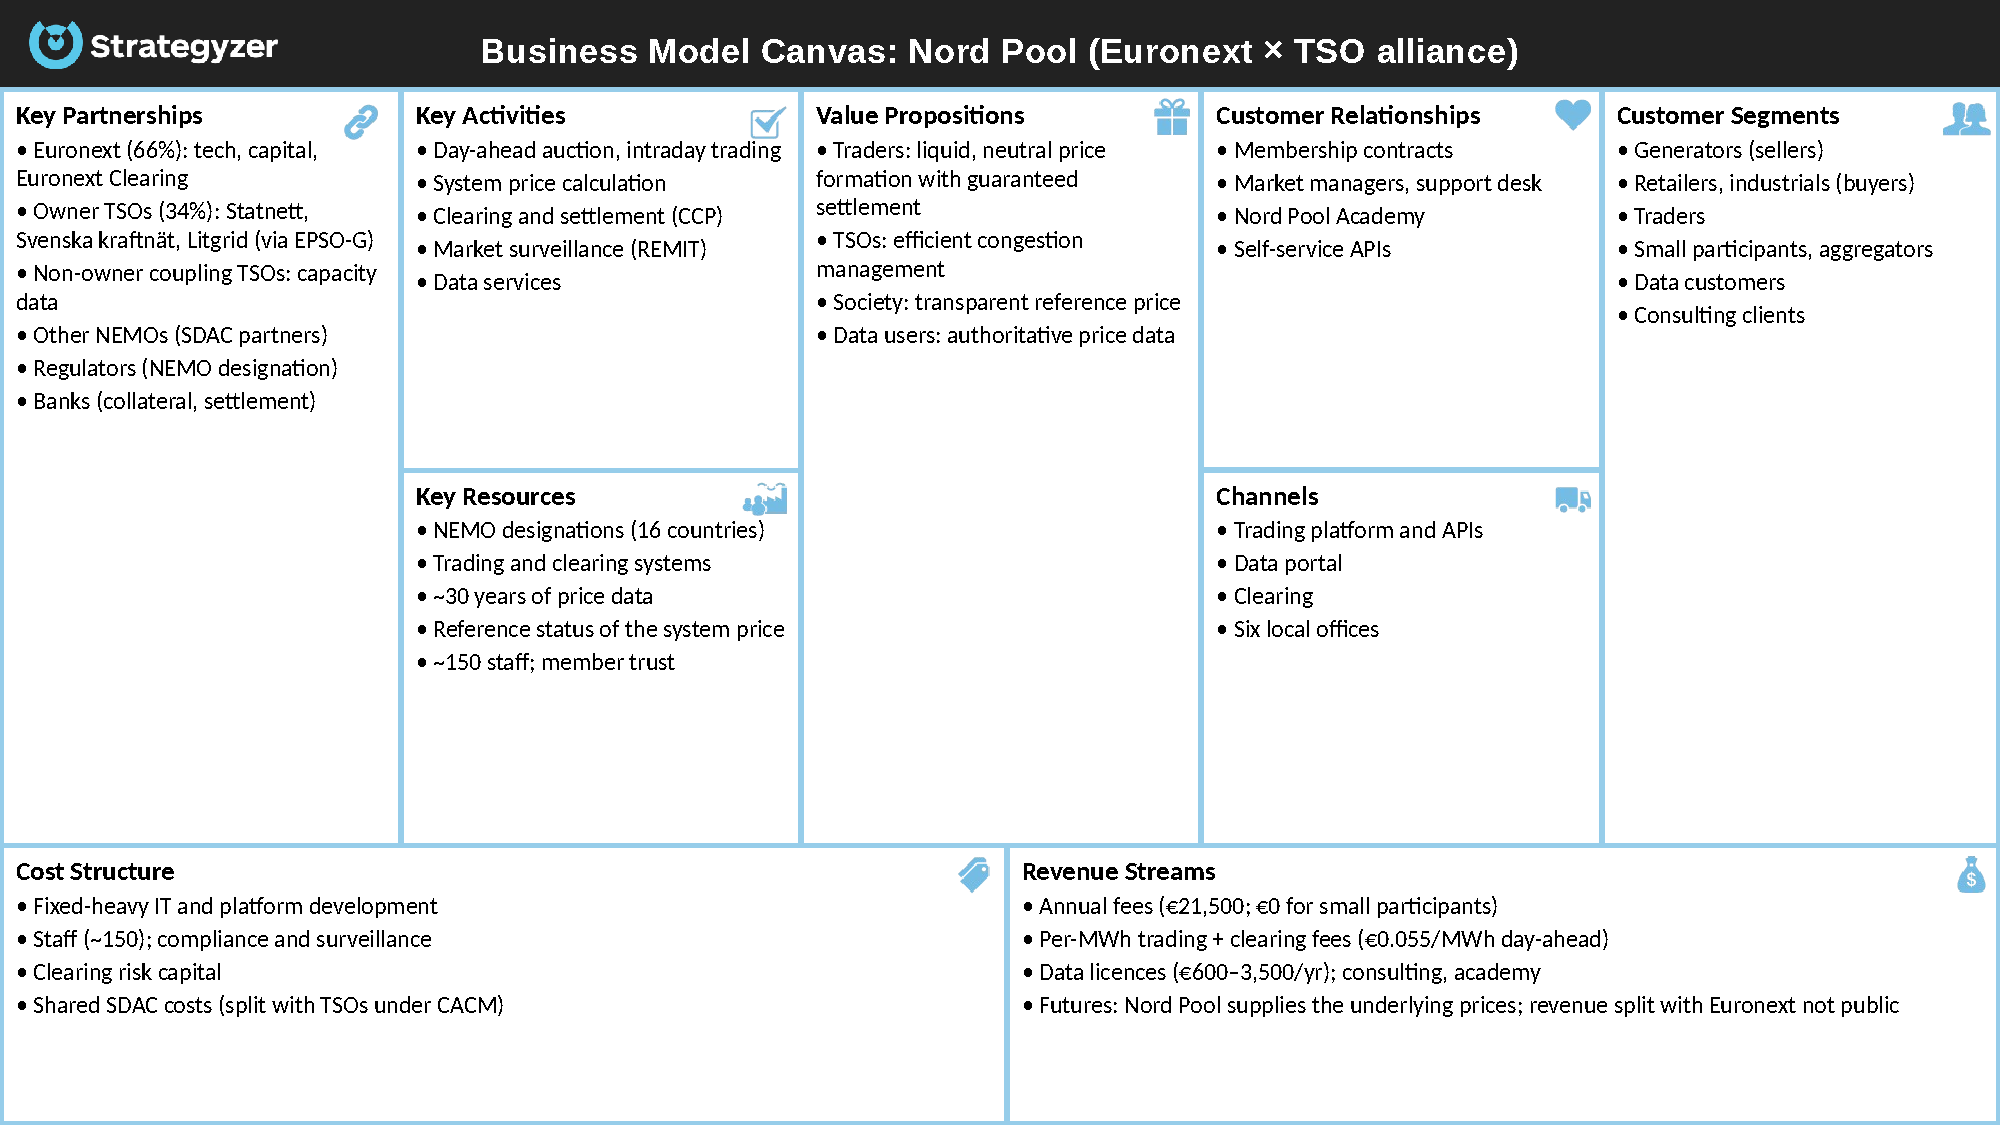
\includegraphics[width=\textheight]{Images/bmc_nordpool.pdf}
\caption{Business Model Canvas for Nord Pool as an alliance platform, made in the course template \citep[building blocks after][Table~19.1]{OverbyAudestad2021}. Prices are from \citet{NPFees2026} and \citet{NPData}; the historical-data price is a 2022 figure \citep{ERR2022}. Staff, offices and countries are from \citet{NPAbout}.}
\label{fig:bmc}
\end{sidewaysfigure}


\textbf{Stakeholder Relationship Model.} The SRM in Figure~\ref{fig:srm} complements the canvas by showing relationships and network effects \citep[Sect.~19.3]{OverbyAudestad2021}. It shows ownership (66/34), capacity data flowing from the TSOs to Nord Pool, fees and licences, the coupling agreement with other NEMOs, and NEMO designation by regulators. Buyers and sellers exert a positive network effect on each other (+/+), as do spot and futures liquidity (+/+), while sellers exert a negative same-side effect on each other ($-$/$-$). The effect of traders on data users runs only one way. The textbook's notation does not cover this case, so we mark it as (+/0). The SRM shows what the canvas hides: the critical dependencies run through actors who do not appear among Nord Pool's customer segments.

% Figure 4: Stakeholder Relationship Model (notation after Øverby & Audestad, Fig. 19.3)
\begin{figure}[ht]
\centering
\begin{tikzpicture}[
  font=\footnotesize,
  st/.style={draw, rounded corners=2pt, align=center, text width=2.6cm, minimum height=0.9cm, fill=white},
  org/.style={st, fill=blue!8, draw=blue!60!black, line width=0.8pt},
  grp/.style={st, double, double distance=1.2pt},
  rel/.style={-{Stealth[length=2mm]}, thick, gray!65!black},
  rel2/.style={{Stealth[length=2mm]}-{Stealth[length=2mm]}, thick, gray!65!black},
  ne/.style={{Stealth[length=2mm]}-{Stealth[length=2mm]}, thick, red!65!black},
  ne1/.style={-{Stealth[length=2mm]}, thick, red!65!black},
  lbl/.style={font=\scriptsize, fill=white, inner sep=1pt, align=center}
]
% top row
\node[st]  (eur)  at (-5.0,3.0) {Euronext};
\node[st]  (reg)  at (-1.8,3.0) {Regulators};
\node[st]  (tsoh) at (1.8,3.0)  {Owner TSOs\\(TSO Holding)};
\node[grp] (ntso) at (5.0,3.0)  {Non-owner TSOs};
% middle row
\node[grp] (epex) at (-5.0,0.2) {EPEX SPOT /\\other NEMOs};
\node[org] (np)   at (0,0.2)    {\textbf{Nord Pool}};
\node[grp] (dat)  at (5.0,0.2)  {Data customers};
% member row
\node[grp] (sel)  at (-3.0,-2.2) {Sellers};
\node[grp] (buy)  at (3.0,-2.2)  {Buyers};
% bottom row
\node[grp] (sml)  at (-5.2,-4.3) {Small participants};
\node[grp] (cons) at (0.6,-4.3)  {Consumers};
\node[grp] (fut)  at (5.2,-4.3)  {Futures traders};

% relationships
\draw[rel]  (eur.south)  -- node[lbl, pos=0.3, below left=1pt]{66\% ownership} (np.north west);
\draw[rel]  (reg.south)  -- node[lbl, pos=0.4, left=2pt]{designation,\\supervision} (np.north);
\draw[rel]  (tsoh.south) -- node[lbl, pos=0.4, left=2pt]{34\% ownership,\\capacity data} (np.north east);
\draw[rel]  (ntso.south west) -- node[lbl, pos=0.3, below right=1pt]{capacity data} (np.east);
\draw[rel2] (epex) -- node[lbl, above=2pt]{SDAC agreement;\\competition} (np);
\draw[rel]  (dat) -- node[lbl, below=2pt]{licence fees} (np);
\draw[rel]  (sel.north east) -- node[lbl, left=3pt]{fees, collateral} (np.south west);
\draw[rel]  (buy.north west) -- node[lbl, right=3pt]{fees, collateral} (np.south east);
\draw[rel]  (cons) -- node[lbl, right=2pt]{retail contracts} (buy.south west);

% network effects
\draw[ne]  (sel) -- node[lbl]{(+/+)} (buy);
\draw[ne]  (sml) -- node[lbl, left=2pt]{(+/+)} (sel);
\draw[ne1] (buy.north east) -- node[lbl, right=2pt]{(+/0)} (dat.south);
\draw[ne]  (fut) -- node[lbl, right=2pt]{(+/+) spot--futures\\liquidity} (buy.south east);
\draw[ne, red!50] (sel.north west) to[out=150,in=210, looseness=6] node[lbl, left]{($-$/$-$)} (sel.south west);
\end{tikzpicture}
\caption{Stakeholder Relationship Model. Double-bordered boxes are groups of similar stakeholders. Grey arrows show relationships (asset exchange, formal agreements), and red arrows show network effects using the SRM notation of \citet[Sect.~19.3]{OverbyAudestad2021}. The one-way effect of traders on data customers, (+/0), extends the textbook notation.}
\label{fig:srm}
\end{figure}

